\documentclass[presentation,xcolor=pdftex,dvipsnames,table]{beamer}\usepackage[]{graphicx}\usepackage[]{color}
%% maxwidth is the original width if it is less than linewidth
%% otherwise use linewidth (to make sure the graphics do not exceed the margin)
\makeatletter
\def\maxwidth{ %
  \ifdim\Gin@nat@width>\linewidth
    \linewidth
  \else
    \Gin@nat@width
  \fi
}
\makeatother

\definecolor{fgcolor}{rgb}{0.345, 0.345, 0.345}
\newcommand{\hlnum}[1]{\textcolor[rgb]{0.686,0.059,0.569}{#1}}%
\newcommand{\hlstr}[1]{\textcolor[rgb]{0.192,0.494,0.8}{#1}}%
\newcommand{\hlcom}[1]{\textcolor[rgb]{0.678,0.584,0.686}{\textit{#1}}}%
\newcommand{\hlopt}[1]{\textcolor[rgb]{0,0,0}{#1}}%
\newcommand{\hlstd}[1]{\textcolor[rgb]{0.345,0.345,0.345}{#1}}%
\newcommand{\hlkwa}[1]{\textcolor[rgb]{0.161,0.373,0.58}{\textbf{#1}}}%
\newcommand{\hlkwb}[1]{\textcolor[rgb]{0.69,0.353,0.396}{#1}}%
\newcommand{\hlkwc}[1]{\textcolor[rgb]{0.333,0.667,0.333}{#1}}%
\newcommand{\hlkwd}[1]{\textcolor[rgb]{0.737,0.353,0.396}{\textbf{#1}}}%
\let\hlipl\hlkwb

\usepackage{framed}
\makeatletter
\newenvironment{kframe}{%
 \def\at@end@of@kframe{}%
 \ifinner\ifhmode%
  \def\at@end@of@kframe{\end{minipage}}%
  \begin{minipage}{\columnwidth}%
 \fi\fi%
 \def\FrameCommand##1{\hskip\@totalleftmargin \hskip-\fboxsep
 \colorbox{shadecolor}{##1}\hskip-\fboxsep
     % There is no \\@totalrightmargin, so:
     \hskip-\linewidth \hskip-\@totalleftmargin \hskip\columnwidth}%
 \MakeFramed {\advance\hsize-\width
   \@totalleftmargin\z@ \linewidth\hsize
   \@setminipage}}%
 {\par\unskip\endMakeFramed%
 \at@end@of@kframe}
\makeatother

\definecolor{shadecolor}{rgb}{.97, .97, .97}
\definecolor{messagecolor}{rgb}{0, 0, 0}
\definecolor{warningcolor}{rgb}{1, 0, 1}
\definecolor{errorcolor}{rgb}{1, 0, 0}
\newenvironment{knitrout}{}{} % an empty environment to be redefined in TeX

\usepackage{alltt}
\usetheme{Hannover}

\usepackage[utf8]{inputenc}
\usepackage[T1]{fontenc}
\usepackage[english, norsk]{babel}
\usepackage{xspace}
\usepackage{booktabs}
\usepackage{rotating}
\usepackage{graphicx}
\setbeamerfont{caption}{size=\scriptsize}







\title[Degenerativ Nakke \\Tromsø, UNN]{\textit{NKR - Degenerativ Nakke} \\
MÅNEDSRAPPORT \\
Tromsø, UNN}
\date{}
\IfFileExists{upquote.sty}{\usepackage{upquote}}{}
\begin{document}
\begin{tiny}

\maketitle

\section{Registreringsoversikter}

\begin{frame}[fragile] {Innhold}
Dette er en sammenstilling av resultater  fra Norsk Kvalitetsregister for Ryggkirurgi, Degenerativ Nakke.
Alle registreringer er basert på registreringer i registeret per rapportdato. Data er hentet rett fra registeret og er ikke kvalitetssikret.
Datoer/årstall er basert på operasjonsdato. Resultatene som vises er i all hovedsak for de siste 12 måneder.
Tidsutvalg for rapportene er spesifisert øverst i hver enkelt figur.

Rapporten viser følgende:
\begin{itemize}
\item Antall registreringer per måned og avdeling.
\item	Registreringsoversikt med antall registreringer av hver skjematype.
\item Andel som får sårdren
\item	Stemmevansker
\item	Svelgvansker
\item	Sårinfeksjon
\item	Fornøydhet med behandlinga på sykehuset
\item	Nytte av operasjonen
\item Forbedring av NDI
\item Forbedring av armsmerter
\item Forbeding av nakkesmerter
\end{itemize}

Dette er bare et lite utvalg resultater. På Rapporteket kan du finne mer spesifikke resultater for disse og mange andre variable.

\end{frame}


\begin{frame}[fragile]

% latex table generated in R 3.4.1 by xtable 1.8-2 package
% Fri Mar 16 10:12:06 2018
\begin{table}[ht]
\centering
\scalebox{0.72}{
\begin{tabular}{lrrrrrrrrrrrrr}
  \hline
 & mar & apr & mai & jun & jul & aug & sep & okt & nov & des & jan & feb & Sum \\ 
  \hline
Aleris Helse AS & 0 & 1 & 3 & 2 & 1 & 1 & 0 & 3 & 1 & 0 & 0 & 0 & 12 \\ 
  Haukeland USH & 12 & 4 & 13 & 6 & 2 & 7 & 9 & 6 & 14 & 9 & 5 & 8 & 95 \\ 
  Oslo, RH & 39 & 25 & 36 & 37 & 6 & 23 & 28 & 20 & 27 & 13 & 3 & 0 & 257 \\ 
  Oslo, Ullevål USH & 28 & 16 & 13 & 12 & 6 & 10 & 6 & 17 & 20 & 13 & 3 & 0 & 144 \\ 
  Oslofjordklin., øst & 11 & 15 & 22 & 12 & 2 & 10 & 13 & 19 & 13 & 12 & 0 & 0 & 129 \\ 
  Oslofjordklinikken Vest & 7 & 2 & 5 & 3 & 5 & 1 & 5 & 4 & 7 & 0 & 0 & 0 & 39 \\ 
  Stavanger USH & 12 & 11 & 13 & 13 & 0 & 11 & 18 & 20 & 16 & 20 & 19 & 1 & 154 \\ 
  Tromsø, UNN & 6 & 5 & 7 & 8 & 1 & 3 & 2 & 6 & 7 & 2 & 5 & 1 & 53 \\ 
  Trondheim, St. Olav & 11 & 8 & 11 & 6 & 3 & 3 & 19 & 11 & 11 & 14 & 15 & 5 & 117 \\ 
  Volvat & 0 & 0 & 0 & 0 & 0 & 0 & 0 & 0 & 0 & 0 & 0 & 0 & 0 \\ 
  Sum & 126 & 87 & 123 & 99 & 26 & 69 & 100 & 106 & 116 & 83 & 50 & 15 & 1000 \\ 
   \hline
\end{tabular}
}
\caption{Antall registereringer (ferdigstilte legeskjema)
                                                          per måned og avdeling, siste 12 måneder.} 
\end{table}


%\scalebox{0.9}{
%\begin{tabular}
%tabAvdSiste12mndUt
%\end{tabular}
%}

\end{frame}


\begin{frame}[fragile]
% latex table generated in R 3.4.1 by xtable 1.8-2 package
% Fri Mar 16 10:12:07 2018
\begin{table}[ht]
\centering
\begin{tabular}{lrrrr}
  \hline
 & Lege & Pasient & Oppf. 3 mnd. & Oppf. 3 mnd. (\%) \\ 
  \hline
Aleris Helse AS & 12 & 12 & 5 & 41.7 \\ 
  Haukeland USH & 95 & 93 & 47 & 61.0 \\ 
  Oslo, RH & 257 & 257 & 167 & 69.3 \\ 
  Oslo, Ullevål USH & 144 & 144 & 77 & 58.8 \\ 
  Oslofjordklin., øst & 129 & 129 & 70 & 58.8 \\ 
  Oslofjordklinikken Vest & 39 & 39 & 17 & 43.6 \\ 
  Stavanger USH & 154 & 154 & 57 & 48.7 \\ 
  Tromsø, UNN & 53 & 53 & 18 & 39.1 \\ 
  Trondheim, St. Olav & 117 & 117 & 42 & 48.3 \\ 
  Volvat & 0 & 0 & 0 &  \\ 
  Sum & 1000 & 998 & 500 & 57.5 \\ 
   \hline
\end{tabular}
\caption{Antall ferdigstilte skjema av hver type per måned og avdeling, for operasjoner
                                  utført siste 12 måneder. For oppfølgingsskjema er antall og andel basert på operasjoner i perioden 2017-03-01 til 2017-12-06.} 
\end{table}

\end{frame}






\section{Prosess}

\begin{frame}[fragile]
\begin{figure}[ht]
\centering
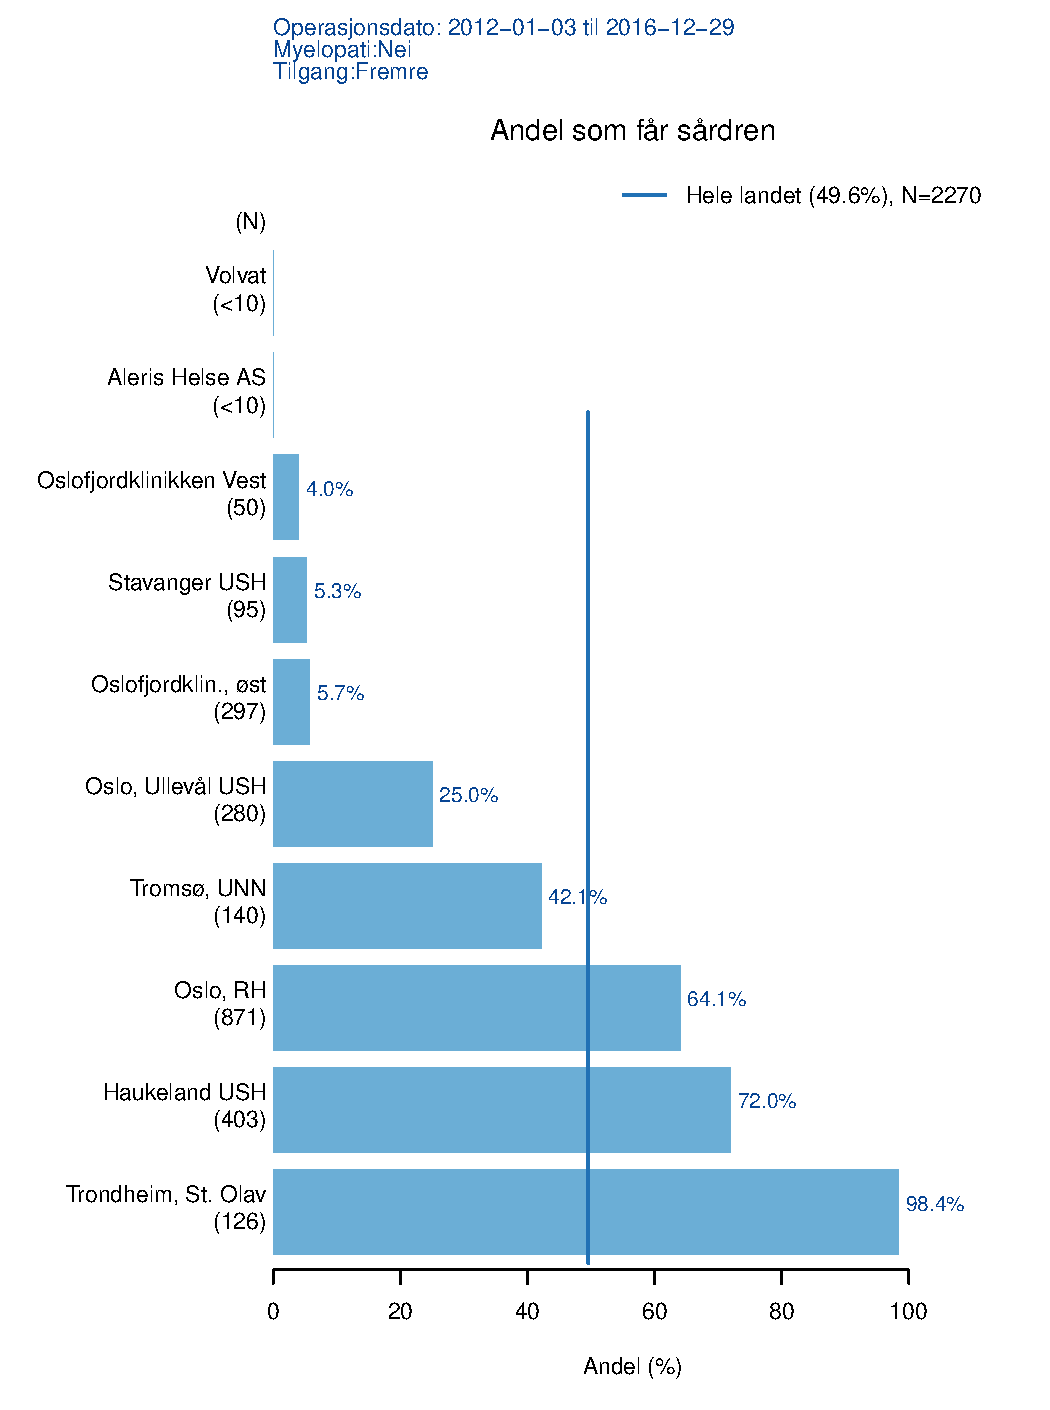
\includegraphics[scale=0.35]{NakkeSaardrenUmFSh.pdf}
\caption[scale=0.3]{Andel pasienter som har fått sårdren. }
\end{figure}
\end{frame}

\begin{frame}[fragile]
\begin{figure}[ht]
\centering
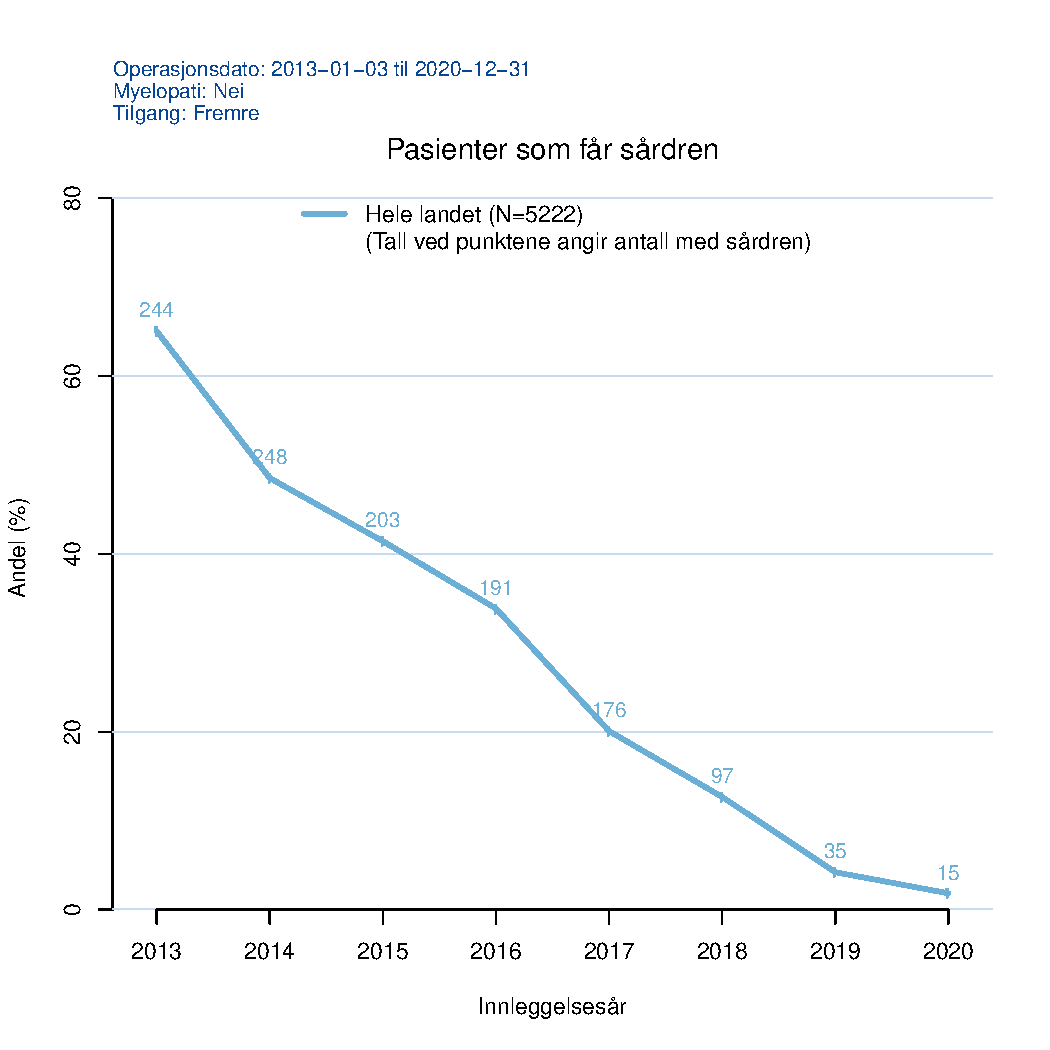
\includegraphics[scale=0.35]{NakkeSaardrenUmFTid.pdf}
\caption{Andel pasienter som har fått sårdren, utvikling over tid. }
\end{figure}
\end{frame}


\section{Komplikasjoner}

\begin{frame}[fragile]
\begin{figure}[ht]
\centering
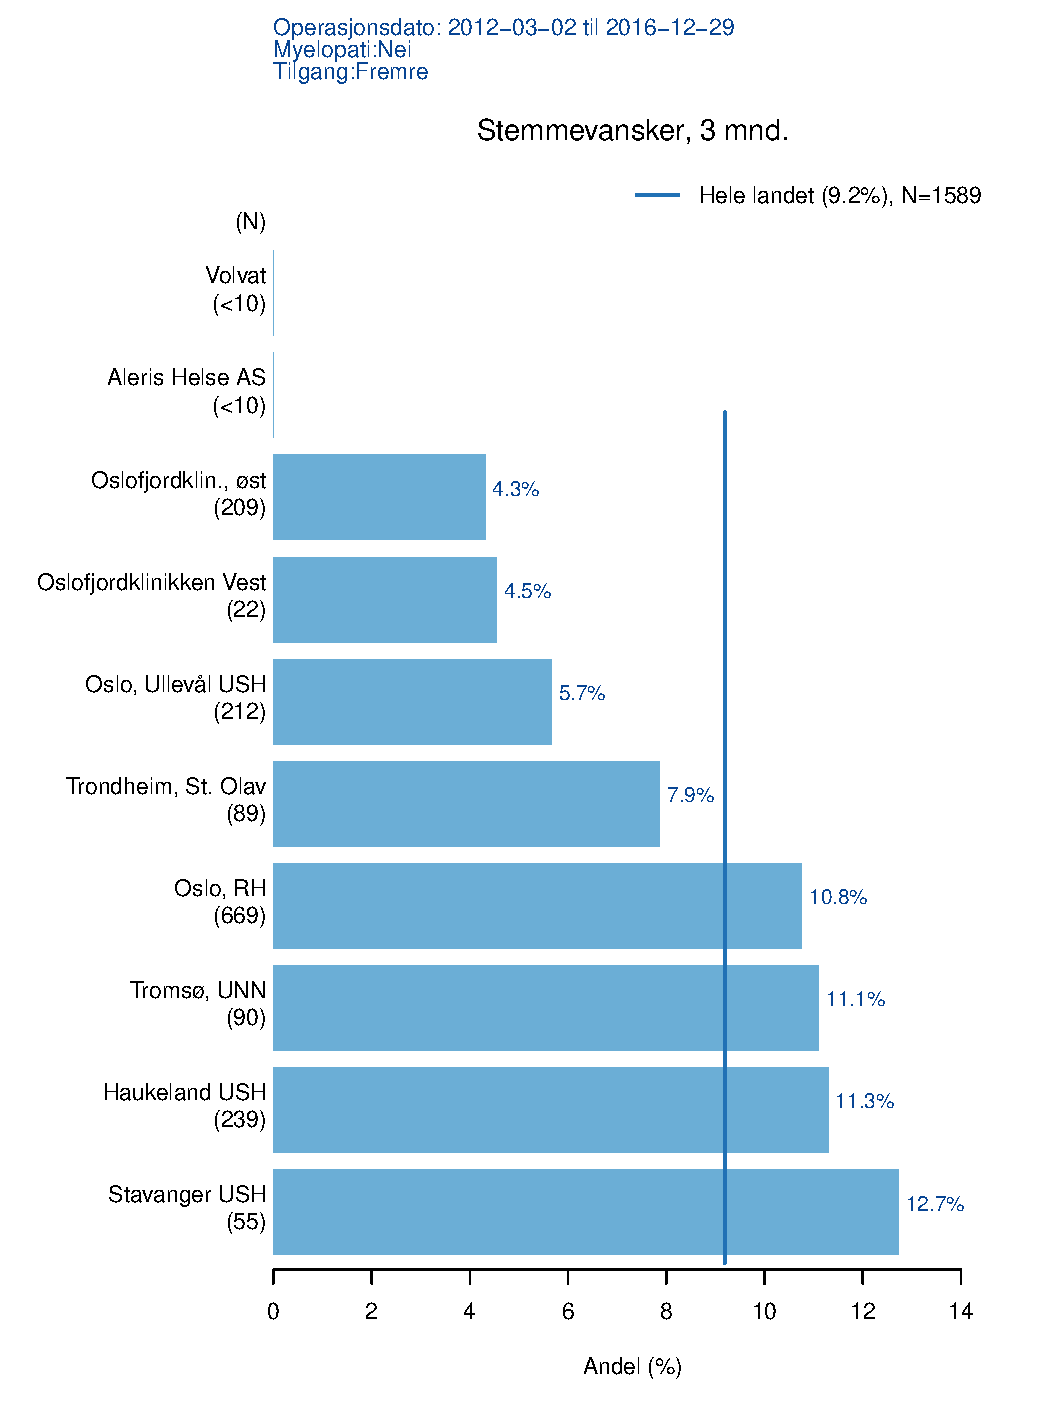
\includegraphics[scale=0.35]{NakkeStemme3mndSh.pdf}
\caption{Stemmevansker, 3 måneder etter operasjon. }
\end{figure}
\end{frame}

\begin{frame}[fragile]
\begin{figure}[ht]
\centering
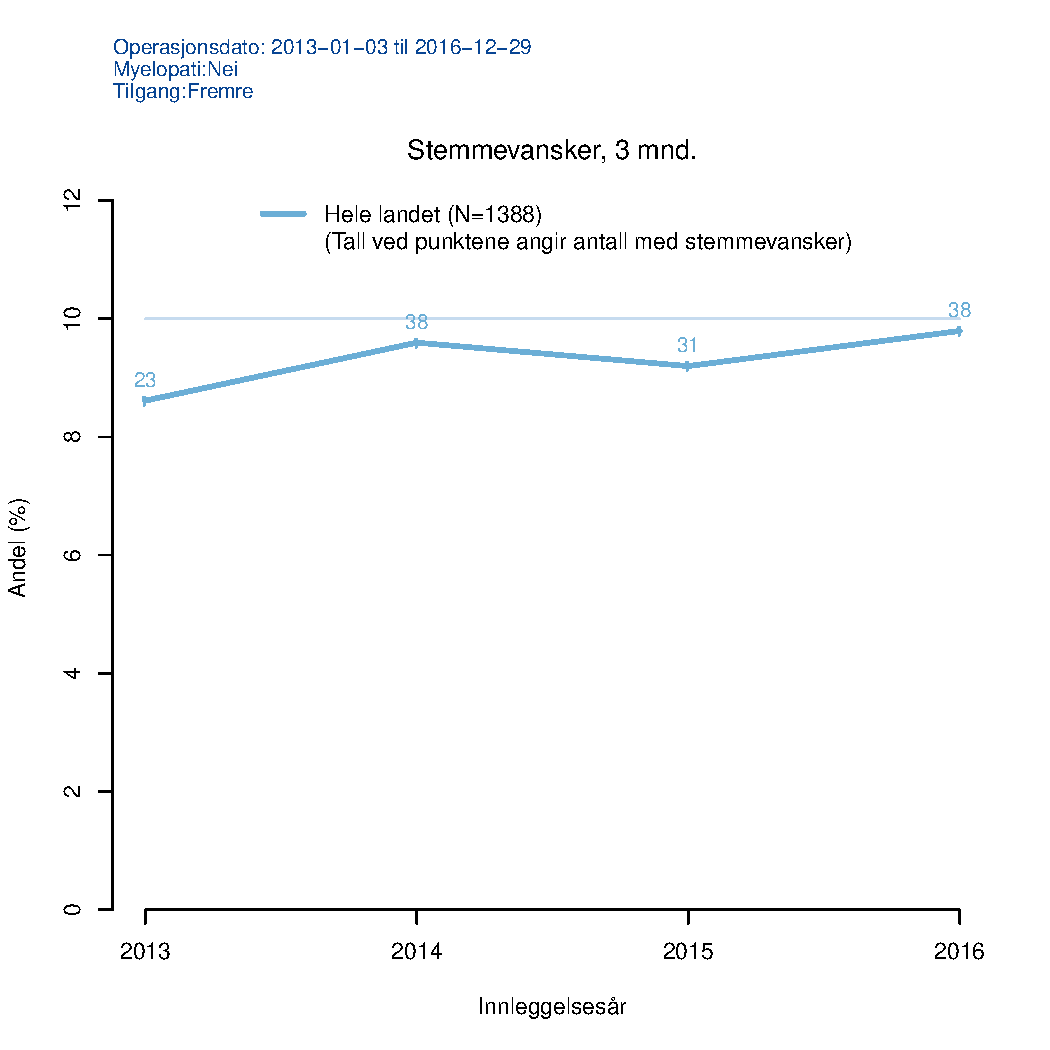
\includegraphics[scale=0.35]{NakkeStemme3mndTid.pdf}
\caption{Stemmevansker, 3 måneder etter operasjon, utvikling over tid. }
\end{figure}
\end{frame}

\begin{frame}[fragile]
\begin{figure}[ht]
\centering
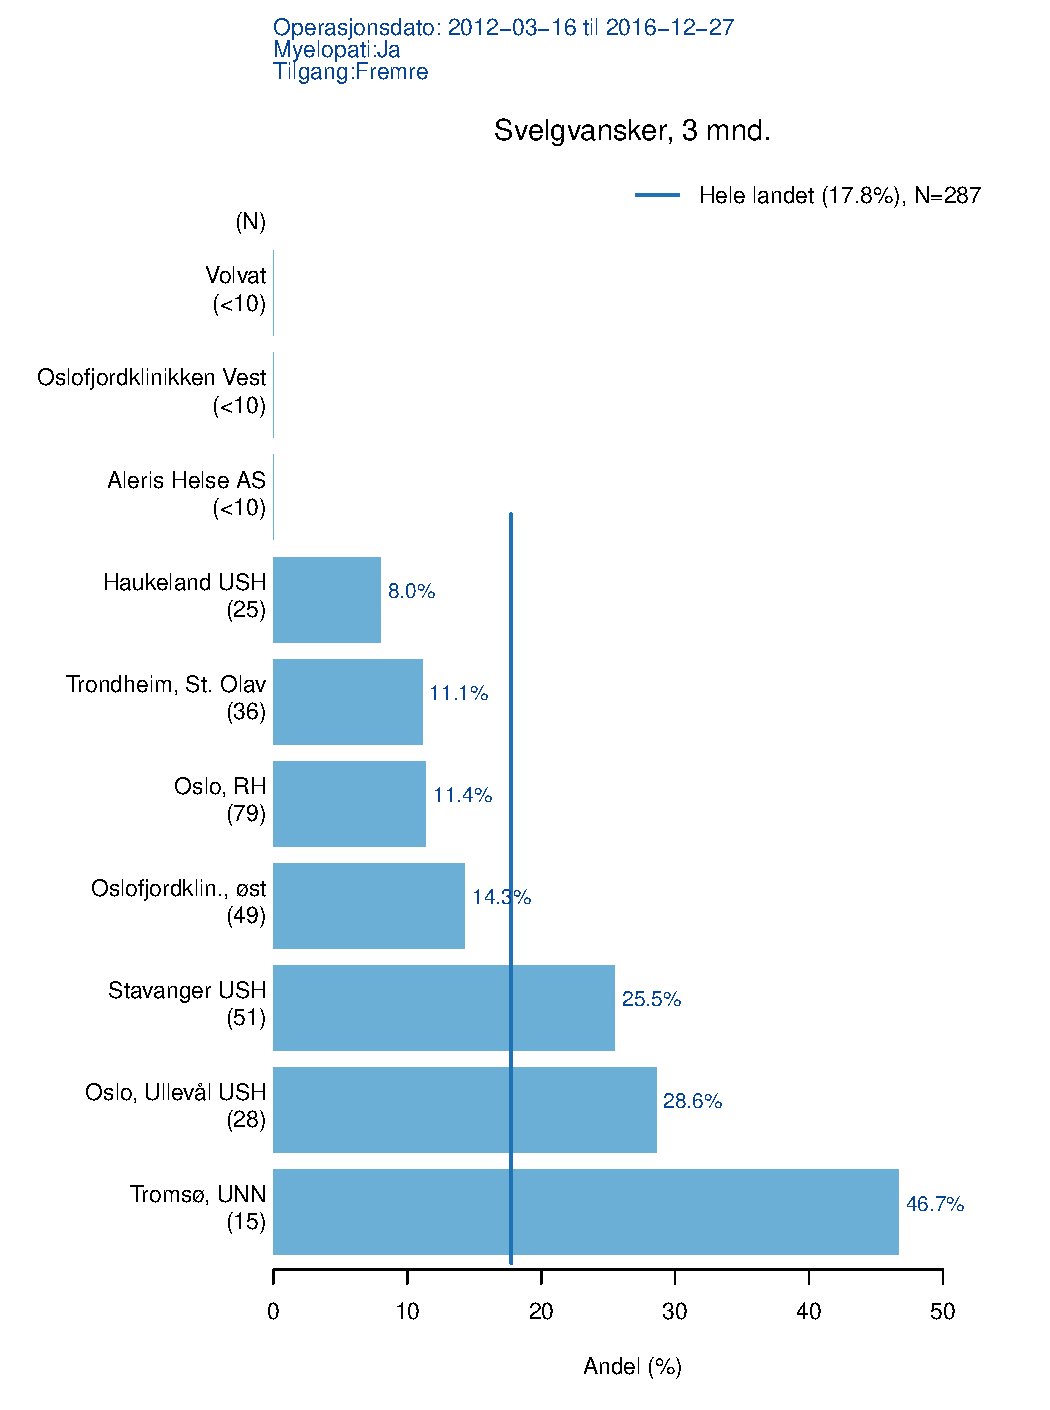
\includegraphics[scale=0.35]{NakkeSvelg3mndSh.pdf}
\caption{Svelgvansker, 3 måneder etter operasjon. }
\end{figure}
\end{frame}

\begin{frame}[fragile]
\begin{figure}[ht]
\centering
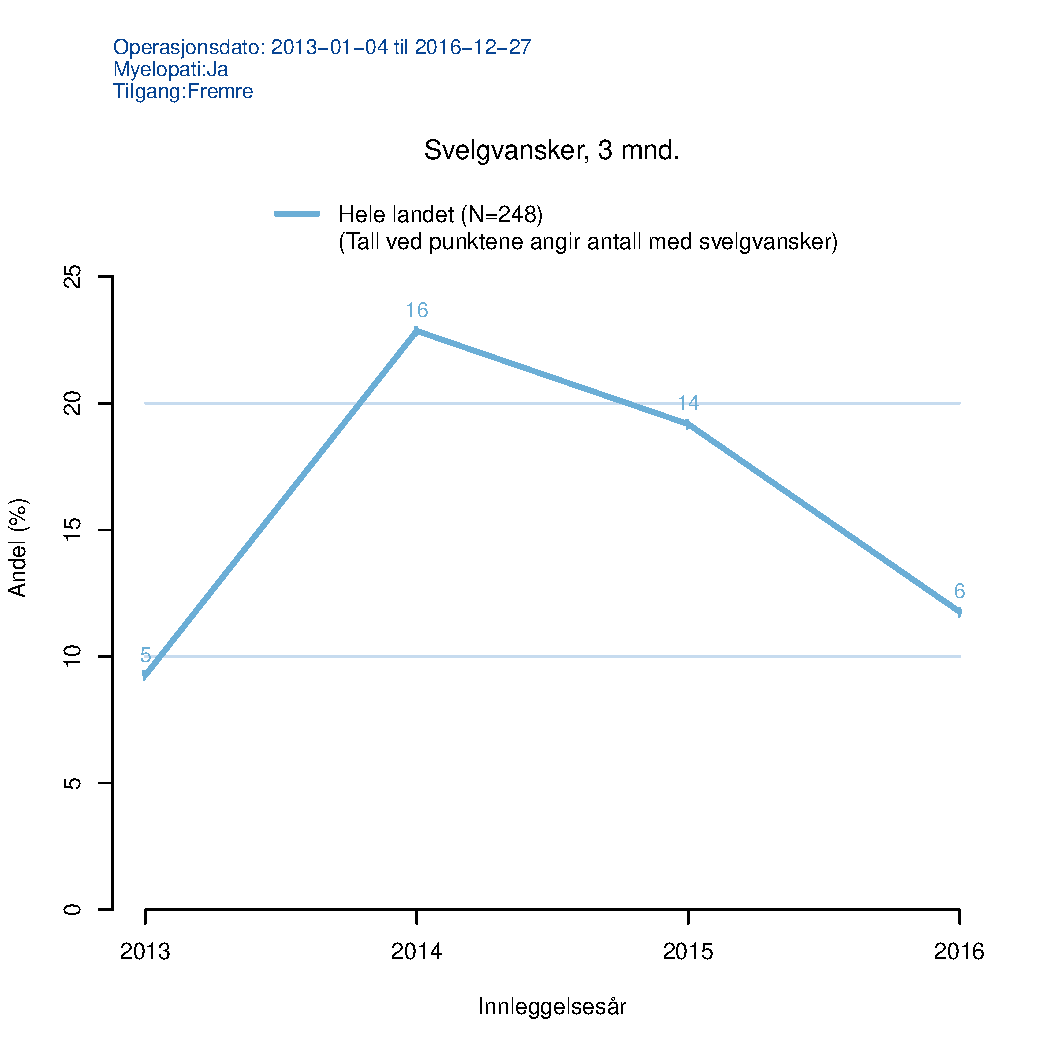
\includegraphics[scale=0.35]{NakkeSvelg3mndTid.pdf}
\caption{Svelgvansker, 3 måneder etter operasjon, utvikling over tid. }
\end{figure}
\end{frame}


\begin{frame}[fragile]
\begin{figure}[ht]
\centering
\includegraphics[scale=0.35]{NakkeKomplinfek3mndSh.pdf}
\caption{Infeksjoner (overfladiske og dype), 3 måneder etter operasjon. }
\end{figure}
\end{frame}


\begin{frame}[fragile]
\begin{figure}[ht]
\centering
\includegraphics[scale=0.35]{NakkeKomplinfek3mndTid.pdf}
\caption{Infeksjoner (overfladiske og dype), 3 måneder etter operasjon. Utvikling over tid. }
\end{figure}
\end{frame}


\section{PROM/PREM, 3 måneder}

\begin{frame}[fragile]
\begin{figure}[ht]
\centering
\includegraphics[scale=0.35]{NDIendr3mndFremUmSh.pdf}
\caption{Gjennomsnittlig forbedring i NDI, fremre tilgang, u/myelopati. }
\end{figure}
\end{frame}

\begin{frame}[fragile]
\begin{figure}[ht]
\centering
\includegraphics[scale=0.35]{NDIendr3mndFremUmTid.pdf}
\caption{Gjennomsnittlig forbedring i NDI, fremre tilgang, u/myelopati. }
\end{figure}
\end{frame}

\begin{frame}[fragile]
\begin{figure}[ht]
\centering
\includegraphics[scale=0.35]{NDIendr3mndBakMmSh.pdf}
\caption{Gjennomsnittlig forbedring i NDI for myelopatipasienter, bakre tilgang.}
\end{figure}
\end{frame}

\begin{frame}[fragile]
\begin{figure}[ht]
\centering
\includegraphics[scale=0.35]{NDIendr3mndBakMmTid.pdf}
\caption{Gjennomsnittlig forbedring i NDI for myelopatipasienter, bakre tilgang.}
\end{figure}
\end{frame}

\begin{frame}[fragile]
\begin{figure}[ht]
\centering
\includegraphics[scale=0.35]{NRSsmerteArmEndr3mndBakMmSh.pdf}
\caption{Gjennomsnittlig forbedring i armsmerte, fremre tilgang u/myelopati.}
\end{figure}
\end{frame}

\begin{frame}[fragile]
\begin{figure}[ht]
\centering
\includegraphics[scale=0.35]{NRSsmerteArmEndr3mndBakMmTid.pdf}
\caption{Gjennomsnittlig forbedring i armsmerte, fremre tilgang u/myelopati.}
\end{figure}
\end{frame}

\begin{frame}[fragile]
\begin{figure}[ht]
\centering
\includegraphics[scale=0.35]{NSRsmerteNakkeEndr3mndSh.pdf}
\caption{Gjennomsnittlig forbedring i nakkesmerte}
\end{figure}
\end{frame}

\begin{frame}[fragile]
\begin{figure}[ht]
\centering
\includegraphics[scale=0.35]{NSRsmerteNakkeEndr3mndTid.pdf}
\caption{Gjennomsnittlig forbedring i nakkesmerte, utvikling over tid.}
\end{figure}
\end{frame}

\begin{frame}[fragile]
\begin{figure}[ht]
\centering
\includegraphics[scale=0.35]{NakkeFornoydBeh3mnd.pdf}
\caption{Pasienter som var helt eller litt fornøyd med behandlinga på sykehuset. }
\end{figure}
\end{frame}

\begin{frame}[fragile]
\begin{figure}[ht]
\centering
\includegraphics[scale=0.35]{NakkeFornoydBeh3mndTid.pdf}
\caption{Pasienter som var helt eller litt fornøyd med behandlinga på sykehuset. Utvikling over tid. }
\end{figure}
\end{frame}


\begin{frame}[fragile]
\begin{figure}[ht]
\centering
\includegraphics[scale=0.35]{NakkeNytteOpr3mndFremUmSh.pdf}
\caption{Pasienter uten myelopati operert med fremre tilgang og som har blitt helt bra eller mye bedre 3 mnd. etter operasjonen. }
\end{figure}
\end{frame}

\begin{frame}[fragile]
\begin{figure}[ht]
\centering
\includegraphics[scale=0.35]{NakkeNytteOpr3mndFremUmTid.pdf}
\caption{Pasienter uten myelopati operert med fremre tilgang og som har blitt helt bra eller mye bedre 3 mnd. etter operasjonen. Utvikling over tid. }
\end{figure}
\end{frame}

\begin{frame}[fragile]
\begin{figure}[ht]
\centering
\includegraphics[scale=0.35]{NakkeNytteOpr3mndBakMmSh.pdf}
\caption{Pasienter med myelopati operert med bakre tilgang og som har blitt helt bra eller mye bedre 3 mnd. etter operasjonen. }
\end{figure}
\end{frame}

\begin{frame}[fragile]
\begin{figure}[ht]
\centering
\includegraphics[scale=0.35]{NakkeNytteOpr3mndBakMmTid.pdf}
\caption{Pasienter med myelopati operert med bakre tilgang og som har blitt helt bra eller mye bedre 3 mnd. etter operasjonen.}
\end{figure}
\end{frame}

\end{tiny}
\end{document}
